%-------------------------------------------------------------------------------
% LATEX TEMPLATE ARTIKEL
%-------------------------------------------------------------------------------
% Dit template is voor gebruik door studenten van de de bacheloropleiding 
% Informatica van de Universiteit van Amsterdam.
% Voor informatie over schrijfvaardigheden, zie 
%                               https://practicumav.nl/schrijven/index.html
%
%-------------------------------------------------------------------------------
%	PACKAGES EN DOCUMENT CONFIGURATIE
%-------------------------------------------------------------------------------

\documentclass{uva-inf-article}
\usepackage[english]{babel}
\usepackage{tikz}
\usepackage{pdflscape}
\usepackage{todonotes}
\usepackage[backend=biber, style=ieee,citestyle=numeric-comp]{biblatex}

\addbibresource{references.bib}

%-------------------------------------------------------------------------------
%	GEGEVENS VOOR IN DE TITEL, HEADER EN FOOTER
%-------------------------------------------------------------------------------

% Geef je artikel een logische titel die de inhoud dekt.
\title{gLTF and Babylon Blendshape integration}

% Vul de naam van de opdracht in zoals gegeven door de docent en het type 
% opdracht, bijvoorbeeld 'technisch rapport' of 'essay'.
% \assignment{}
% \assignmenttype{}

% Vul de volledige namen van alle auteurs in en de corresponderende UvAnetID's.
\authors{Jari Andersen}
% \uvanetids{}

% Vul de naam van je tutor, begeleider (mentor), of docent / vakcoördinator in.
% Vermeld in ieder geval de naam van diegene die het artikel nakijkt!
% \tutor{}
% \mentor{}
% \docent{}

% Vul hier de naam van je tutorgroep, werkgroep, of practicumgroep in.
% \group{SignLab, VisualisationLab}

% Vul de naam van de cursus in en de cursuscode, te vinden op o.a. DataNose.
% \course{}
% \courseid{}

% Dit is de datum die op het document komt te staan. Standaard is dat vandaag.
\date{\today}

%-------------------------------------------------------------------------------
%	VOORPAGINA 
%-------------------------------------------------------------------------------

\begin{document}
\maketitle
\tableofcontents
\newpage
%-------------------------------------------------------------------------------
%	INHOUDSOPGAVE EN ABSTRACT
%-------------------------------------------------------------------------------
% Niet toevoegen bij een kort artikel, zeg minder dan 10 pagina's!

%TC:ignore
%\tableofcontents
%\begin{abstract}
%\end{abstract}
%TC:endignore

%-------------------------------------------------------------------------------
%	INHOUD
%-------------------------------------------------------------------------------
% Hanteer bij benadering IMRAD: Introduction, Method, Results, Discussion.
\section{Introduction}
Integrating blendshapes/morphtargets onto an avatar is of the utmost importance for displaying whole body animations. The integration of it however, differs significantly depending on what file format and what engine you are using. In our project to display animations in Babylonjs, we will need to use the gLTF file format (FBX is not supported in Babylon). Getting the blendshapes to work in this format however, proved to be a difficult task, similarly integrating the blendshapes into the Babylon engine was also far from trivial.

In this small report I will go over the difficulties and a (somewhat) final pipeline to achieve an integration.

\section{FBX to gLTF blendshapes}
Coming out of Unreal Engine, we have exported every animation as FBX in our previous projects. However, Babylon requires us to use the gLTF standard. Eventhough we have the ability to export the animations as gLTF through Unreal Engine, we have opted to use other software to convert the FBX to gLTF. Why we do that will become more clear in the following sections.

\subsection{Current support in gLTF}
gLTF, short for "GL Transmission Format," is an open standard maintained by the Khronos Group, aimed at efficient transmission and loading of 3D scenes and models. It's designed to be a lightweight, interoperable format for exchanging rich 3D content between different tools, applications, and platforms. gLTF files can store 3D models, animations, textures, and other scene-related data.

gLTF supports blendshapes for 3D animations. However, there are some flaws in the manner that they have standardized the blendshapes. Currently, blendshapes are implemented such that they can only be accessed through an index value\cite{bsdocu}. The absence of standardized blendshape names poses a notable challenge for users. While gLTF allows saving blendshape data, the lack of standardized naming conventions means that blendshapes are only identifiable by their index, rather than by descriptive names like ``eyeblinkleft" or ``jawopen".

The community has repeatedly requested support for named blendshapes, recognizing the significant workflow improvements it would bring \cite{gitmorphnames}. Unfortunately, supporting this in gLTF itself as a feature has yet to be implemented, making working with blendshapes more cumbersome than necessary.

Various implementors of gLTF have taken it onto themselves to add support for blendshape names \cite{facebookincubatorgLTF, Maya2glTF, threegLTF, babylongLTF}. They use a workarounds, utilizing the "extra" field to map blendshape indices back to their corresponding names. While this workaround provides a solution, it's not universally supported across all software, as it deviates from the standard gLTF specification.

In the next section, I'll delve into the software landscape and detail my experiences with various tools while striving to leverage blendshapes within the gLTF format.

\subsection{Unreal, Blender, 4D cinema, ASPose, FBX2glTF, COCOs}
In a best case scenario, we would export the animation data through Unreal Engine in the gLTF format and the blendshapes would work immediately. Sadly, the exported gLTF or GLB data from Unreal Engine does not contain the blendshapes. We can see this by importing the data into \url{https://sandbox.babylonjs.com/}, and inspecting the mesh morphtargets. Therefore, we will need to get the animation data as FBX from Unreal Engine, which contains blendshapes, and then convert it to gLTF.
Table \ref{tab:conversiontable} goes into detail about various conversion methods that I have tried out.

There are two moments when we can lose blendshapes. Either on import into the software (it does not support FBX blendshapes), or on export converting the FBX to gLTF (it does not support conversion of FBX blendshapes or doesn't support blendshapes al together).

\begin{table}[ht]
\centering
\begin{tabular}{l|l|l|l|p{0.3\linewidth}} 
\textbf{Origin}  & \textbf{Conversion method} & \textbf{Blendshapes} & \textbf{Textures} & \textbf{Extra info}                                                                                 \\\hline
UE GLB  & N/A               & No          & Yes      &                                                                                            \\\hline
UE GLTF & N/A               & No          & Yes      &                                                                                            \\\hline
UE FBX  & COCOS to gltf     & Yes         & No       & Lots of warnings and errors with gLTF validation.                                          \\\hline
UE FBX  & nodejs conversion & No          & No       &                                                                                            \\\hline
UE FBX  & ASPOSE to GLB     & No          & No       & ASPOSE is online converter, everything dies even skeleton                                  \\\hline
UE FBX  & ASPOSE to GLTF    & No          & No       & ASPOSE is online converter, everything dies even skeleton                                  \\\hline
UE FBX  & Blender           & No          & No       & The FBX import into Blender already loses the blendshapes.                                 \\\hline
UE FBX  & NPM fbx2gltf      & Yes       & No       & The meshes contain blendshapes, but they are renamed to morphtarget01, morphtarget02, etc. \\\hline
UE FBX  & 4D Cinema         & No          & No       & The FBX import contains the blendshapes, but the conversion loses them.                   
\end{tabular}
\caption {A conversion table for FBX to gLTF, taking into account blendshapes and textures.} \label{tab:conversiontable} 
\end{table}

\subsection{COCOs and gLTFtransform to Babylon}
Table \ref{tab:conversiontable} shows us that options COCOs FBX-glTF-conv\footnote{\url{https://github.com/cocos/FBX-glTF-conv}} and FBXX2gLTF are the only options to retain blendshapes. The latter however, forces us to figure out what the mapping of the index for the blendshape is with the \textit{renamed} blendshape. This seems like a foolhardy quest when the former offers us the blendshapes with correct names. The COCOs converter comes with its own hurdle. When importing a model that comes from COCOs into the Babylon sandbox, we see that there are many warnings and errors located by the gLTF validator. Ignoring these warnings and using the animations and meshes in Babylon, we suspect that these warnings slow down the load times in Babylon. Therefore we have to fix these warnings (or test further with suppressing warnings). The validator tells us precisely what is wrong with the gLTF file, but nobody feels like fixing 8000+ warnings by hand. Luckily, automated gLTF fixers exist. gLTF Transform\footnote{\url{https://gltf-transform.dev/}} offers such a service, getting rid of all the errors.

\subsection{Textured mesh}
When we export the FBX out of Unreal Engine, we are missing textures. Looking further into this, it becomes clear that it is standard to export the textures separately and later on reapply them to the mesh. In the Babylon Sandbox, we can import the textures after importing the model, and reapply them to the model. Then we export the model as GLB and we are able to use that file in our Babylon projects.

It is important to note that we will only need to do this for each avatar and not for each animation.

\section{Babylon Animation pipeline}
After finally getting a working gLTF file containing all the animations, and blendshapes we are done. NOT! After importing a mesh with animations together, we see that the blendshapes and skeletal animations are working. When importing the mesh separately from the animations however, skeletal animations are present but blendshape animations aren't. We do have so called ``morphtargetmanagers" that contain all blendshapes and animation keys. So what is going on? Babylon forgot to map the blendshape animations after importing the animations.

In order to fix this we have to do a retarget for the animation by hand. Luckily, we know that the source and target skeletons and meshes are the same for the animation retarget. This means that there is no need for calculating relative rotations. A simple mapping is all we need.

How to do this mapping for bones is straightforward\cite{babForum}. And after further inspecting the all the targets from the AnimationGroup clone function\footnote{\url{https://doc.babylonjs.com/typedoc/classes/BABYLON.AnimationGroup\#clone}}, it is also clear how we would read a blendshape and add retarget it.
Figure \ref{fig:mtm} displays the code snippet on retargeting the blendshapes in Babylon. It is important to note that we iterate over multiple morphtargetmanagers (mtm) because multiple sub meshes hold blendshapes (we have eyes, tongue, teeth, and the rest of the face separated).

\begin{figure}[hbt!]
    \centering
    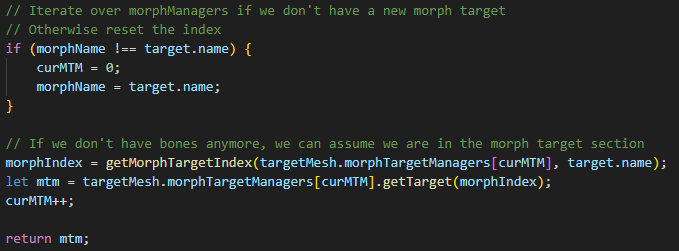
\includegraphics[width=0.7\textwidth]{imgs/mtm.png}
    \caption{Code snippet on retargeting blendshapes}
    \label{fig:mtm}
\end{figure}

After applying the re-mapping, we finally have blendshapes working.

\section{Pipeline}
How does the final pipeline look summarized:
\begin{center}
We export the animations as FBX through Unreal Engine (this ensures that the blendshapes are present). We use COCOs FBX-glTF-conv tool to convert the FBX to gLTF. Then we fix all the errors by using the gLTFtransform tool. We import the textured mesh and animations separately into Babylon. We retarget/remap the animation onto the textured mesh.
\end{center}

\section{Troubleshoot}
In my efforts to retarget the animation onto the mesh I came across some weird behaviour. In this section I will further discuss these.

\subsection{No targets in clone}
When using a mesh, and importing an animation, I came across an issue where I had no targets in the clone function (where I do the retargeting). Tracing this code, you might say that it is the animation importers fault for not adding the targets, but the animation not having any targets actually makes sense. The imported animation has a lot of animation keys and values, but no target because it is not driving any skeletalmesh. Therefore, you cannot use the clone function to do retargeting on different skeletalmeshes (or differently converted/imported skeletalmeshes).

%-------------------------------------------------------------------------------
%	REFERENTIES
%-------------------------------------------------------------------------------

\printbibliography

%-------------------------------------------------------------------------------
%	BIJLAGEN 
%-------------------------------------------------------------------------------

%TC:ignore
% \appendix 
% \section{Bijlage {\LaTeX} code}
% Bijgevoegd zijn de \textattachfile{main.tex}{code} en 
% \textattachfile{references.bib}{bibliografie}.
%TC:endignore

%-------------------------------------------------------------------------------
\end{document}